This research presented a method to process point cloud files, mesh them via panoramic projection, and convert them to textured 3D panorama meshes. Furthermore, it examined whether this method creates useful meshes for artists, by testing it in a real world use case with the goal to reconstruct the historic Pellerhaus Nürnberg. This chapter discusses results and gives an outlook of future work.

\section{Conclusion}

To conclude, we would like to summarize the work, mention its limitations, and present the contributions made by this research.\\

This project was begun with the goal of finding a way for Blender artists to work with laser scanner point clouds in Blender. Blender cannot display colored 3D point clouds in its viewport. Therefore, this required finding a novel method to make point clouds available to artists who wish to work with such data in Blender. We propose a conversion from laser scanner point clouds to textured polygon meshes, because those geometric shapes can be viewed and rendered in Blender. Due to the characteristics of laser scanner devices, environments are sampled in a sphere. Projecting the point samples onto a two-dimensional grid simplifies the process to connect those points and determine texture coordinates. The 3D information can be retrieved by applying the inverse transform to this grid. The 3D mesh is then exported to a commonly used file format to exchange geometric information between applications.

\subsection{Mesh generation}

The generated mesh was evaluated by using it in an artistic project. The goal of this project was to create the modern and historic facades of the Pellerhaus Nürnberg based on the generated 3D panoramas. The goals of this project have been met. First, creating 3D panoramas from point clouds solves the issue that Blender cannot display point clouds and therefore enables artists to work with LiDAR data. Second, the generated meshes have been helpful in producing 3D models of the Pellerhaus Nürnberg.\\

The limitations of this project are mostly related to the quality of the generated mesh. The generated mesh is good enough to provide artists a three-dimensional reference of a particular environment, but it is not perfect. A perfect mesh would have perfectly flat surfaces, for instance. This can only be achieved with almost no quantization of the image files, e.g. by using floating-point values for the pixel data or by using the original point data instead of reprojecting the panorama images. This is currently not implemented in the PC2B prototype due to its memory management, though PC2B can be optimized to improve the generated meshes. For the purpose of this research, the results are satisfying.


\subsection{Handling non-LiDAR data}

Although this research was aimed at investigating point clouds generated by laser scanners, we did experiment with other point cloud generators as well. There are additional ways to produce point clouds, such as Photogrammetry or Depth Cameras. The more points they generate, the better. We have tested our algorithm on both of those point cloud types. We found that our algorithm works well with non-LiDAR data. Photogrammetry point clouds are meshed as follows:

\begin{figure}[h]
	\centering
	\begin{subfigure}[b]{0.49\textwidth}
		\centering
		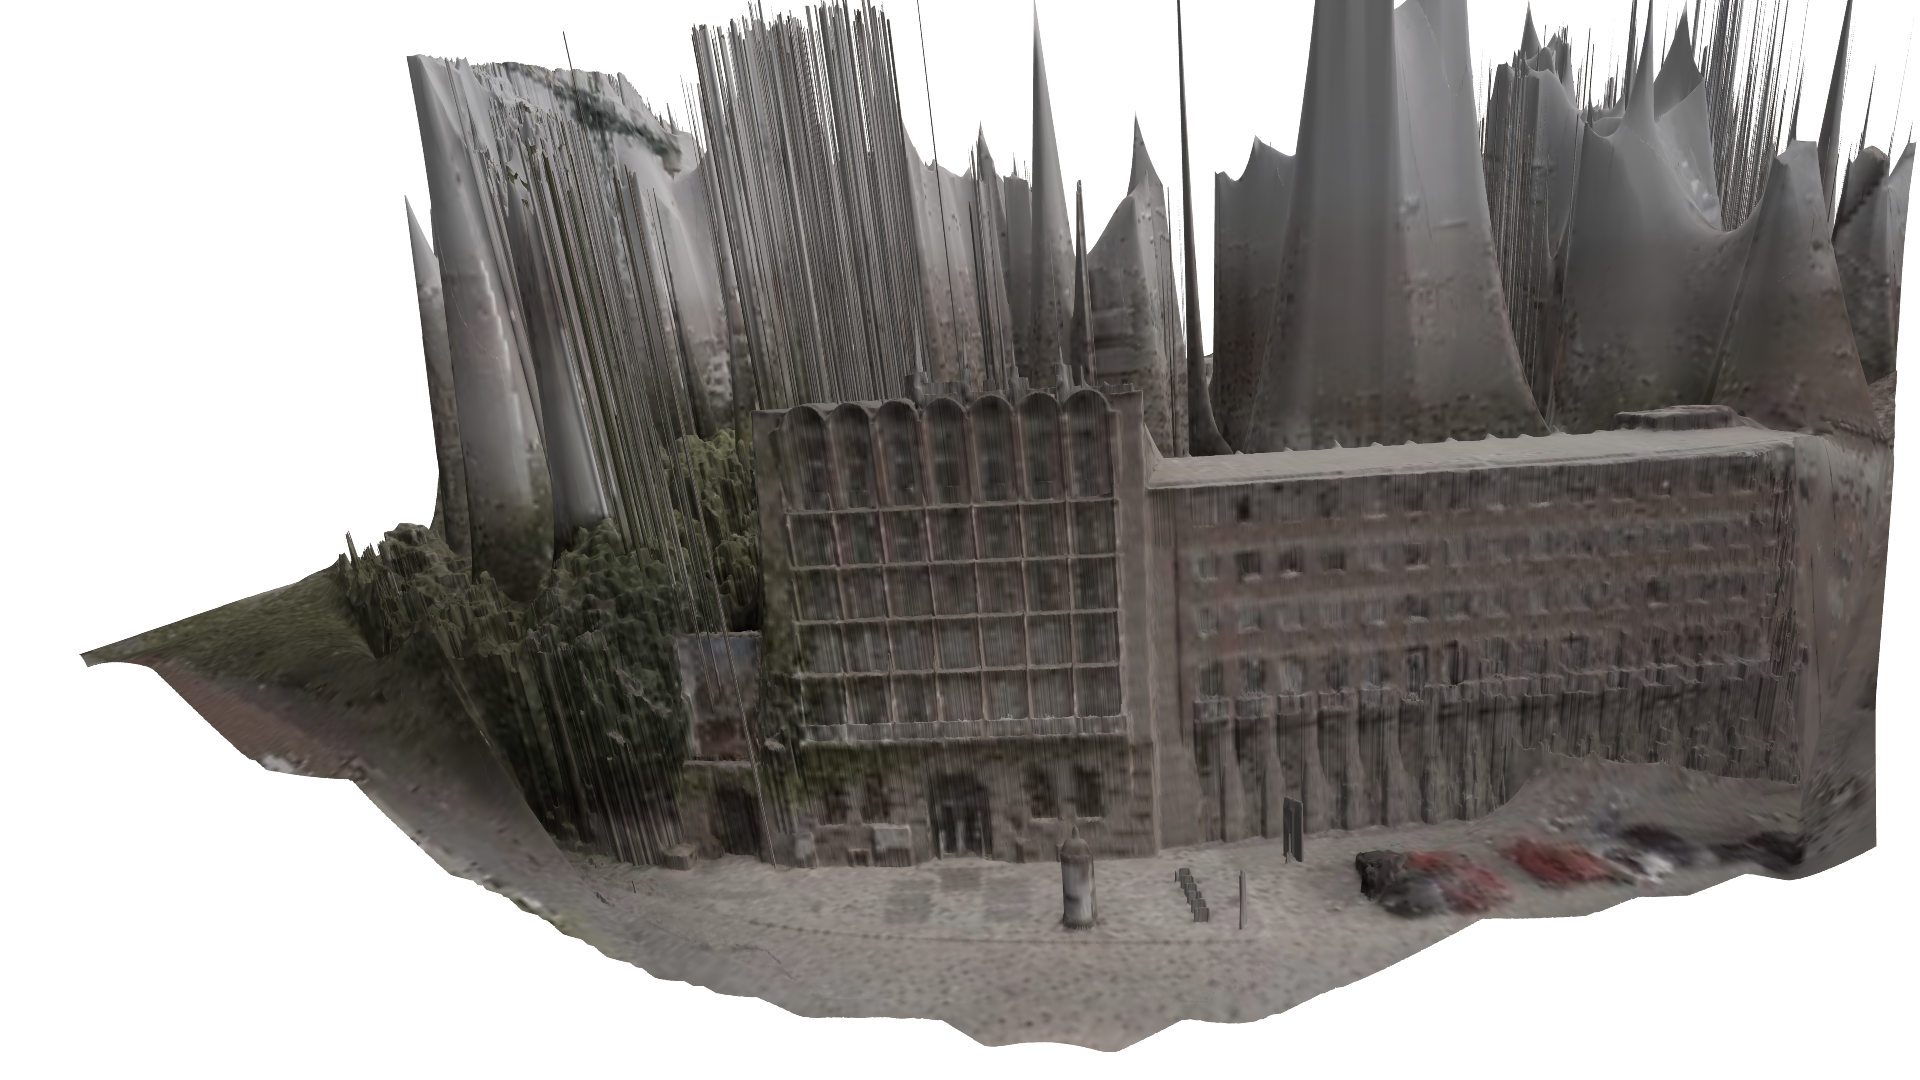
\includegraphics[width=\textwidth]{Conclusion_Meshing_Photoscan.png}
		\caption{Agisoft Photoscan Pro meshing}
		\label{fig:conclusion_meshing_photoscan}
	\end{subfigure}
	\hfill
	\begin{subfigure}[b]{0.49\textwidth}
		\centering
		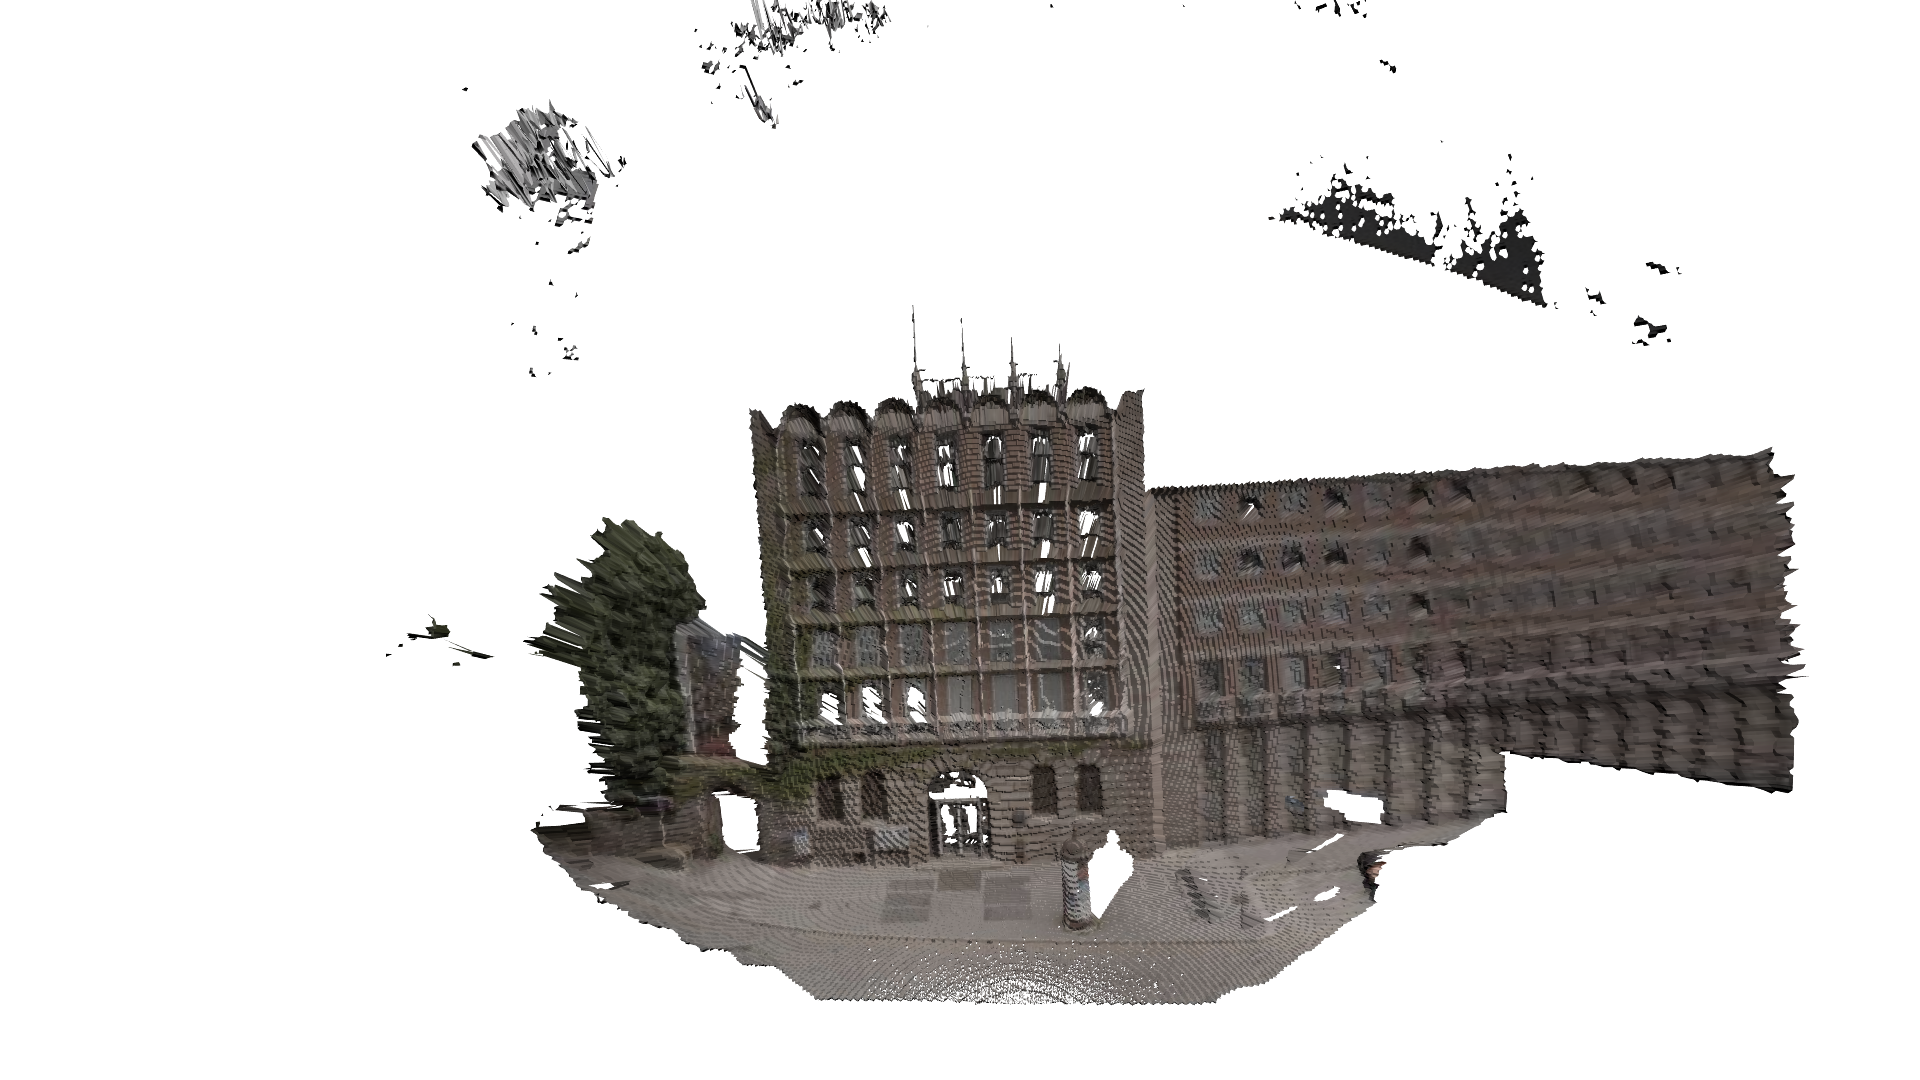
\includegraphics[width=\textwidth]{Conclusion_Meshing_PC2B.png}
		\caption{PC2B meshing}
		\label{fig:conclusion_meshing_pc2b}
	\end{subfigure}
	\caption{Comparison of meshing in Photoscan vs. PC2B}
	\label{fig:conclusion_meshing_photoscan_vs_pc2b}
\end{figure}

\pagebreak

Additionally, we examined the output of a Depth Camera, namely the Asus Xtion Pro Live. Mrs. Eichhorn, a fellow student finishing her bachelor's degree in October 2015, teamed up with us to study ways that our present research can be used in combination with her's. The title of her research paper reads "Selbstständige Navigation eines autonomen Roboters mittels 3D-Tiefensensor" (which translates into English as "Independently navigating an autonomous robot employing a 3D depth sensor", see Eichhorn 2015 \parencite{anja_eichhorn}).\\

\begin{figure}[h]
	\centering
	\begin{subfigure}[b]{0.49\textwidth}
		\centering
		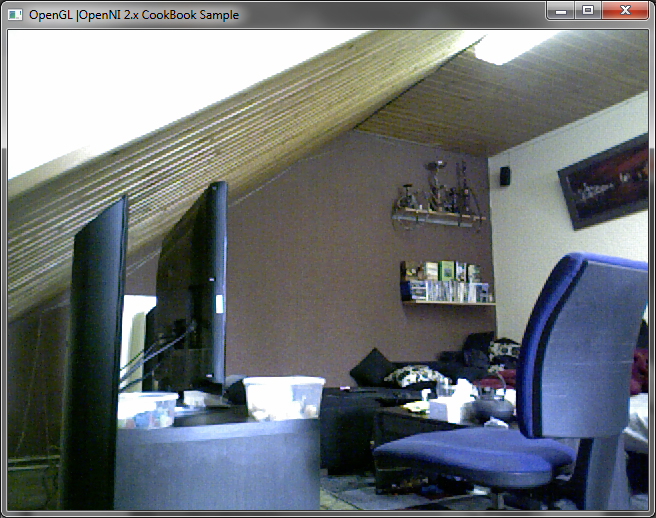
\includegraphics[width=\textwidth]{Conclusion_Szenario1_color.jpg}
		\caption{Color image}
		\label{fig:conclusion_depth_camera_color}
	\end{subfigure}
	\hfill
	\begin{subfigure}[b]{0.49\textwidth}
		\centering
		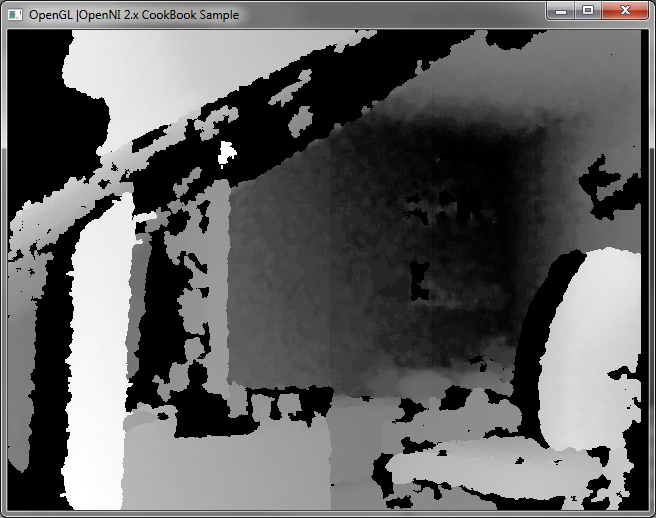
\includegraphics[width=\textwidth]{Conclusion_Szenario1_depth.jpg}
		\caption{Depth image}
		\label{fig:conclusion_depth_camera_depth}
	\end{subfigure}
	\caption{Depth Camera images}
	\label{fig:conclusion_depth_camera_images}
\end{figure}

While we thought about ways to make use of 3D panoramas to help the robot understand its environment, she was asked to provide a point cloud file to see how PC2B would process it. She wrote a custom tool to save the output of a depth sensor to an .xyz file which is compatible with the PC2B converter software. This is the result of this data:\\

\begin{figure}[h]
	\centering
	\begin{subfigure}[b]{0.54\textwidth}
		\centering
		
\includegraphics[width=\textwidth]{Conclusion_PC2B_depthmap.jpg}
		\caption{PC2B depth map panorama (Note: flipped)}
		\label{fig:conclusion_depth_camera_pc2b_panorama}
	\end{subfigure}
	\hfill
	\begin{subfigure}[b]{0.45\textwidth}
		\centering
		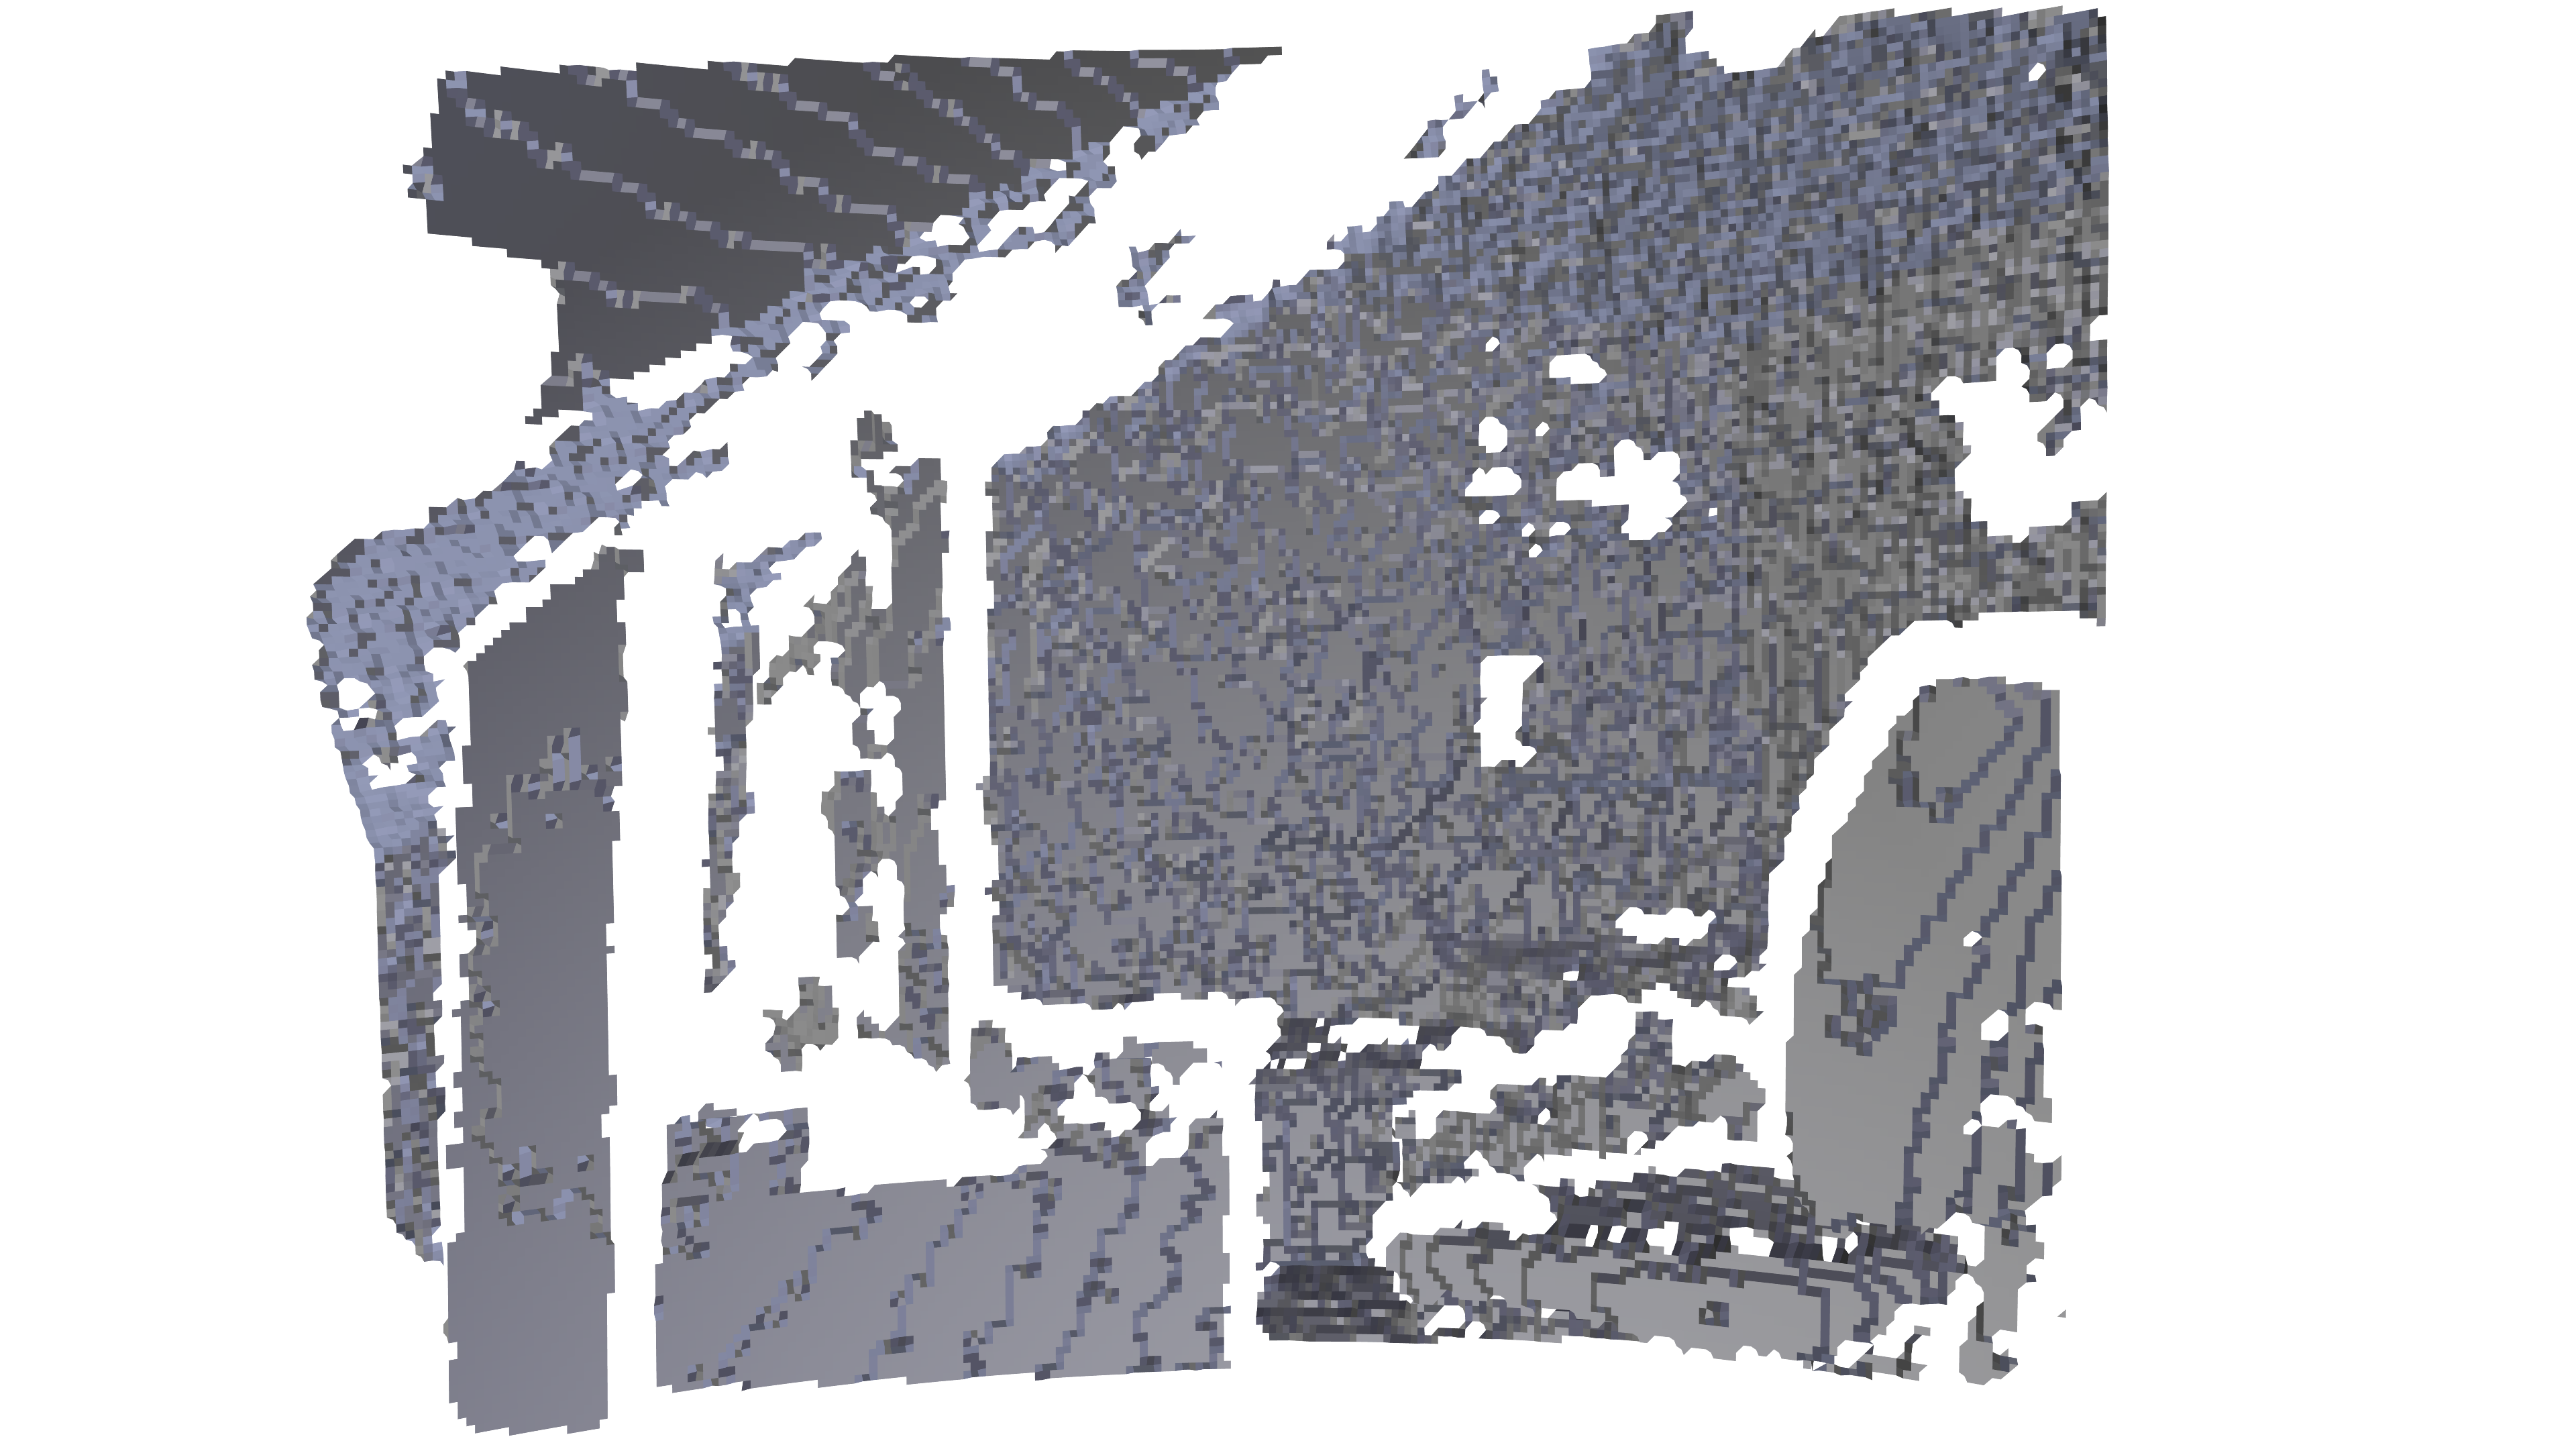
\includegraphics[width=\textwidth]{Conclusion_DepthCamera_PC2B.png}
		\caption{PC2B meshing}
		\label{fig:conclusion_depth_camera_pc2b_meshing}
	\end{subfigure}
	\caption{Meshing of Depth Cameras with PC2B}
	\label{fig:conclusion_depth_camera_meshing}
\end{figure}




The results demonstrate that it is possible to generate 3D panoramas from depth sensors as well. The test data has 77,361 points and is processed in 3297 milliseconds for a quadruple resolution set in the PC2B converter. We plan to continue exploring the use of PC2B for her purpose.


\section{Future Work}

In this section we would like to present further ideas of how PC2B and the 3D models can be used in other fields of application.

\subsection{Improving memory management and performance}

Naturally, bug fixes, optimizations, and a more sophisticated software architecture are important to move from a prototype status to a mature product. We learned a great deal about the weaknesses and strengths of the underlying algorithms and gained the knowledge to decide what parts need to be optimized. The source code of this software tool will remain open, so anyone who would like to learn from it or contribute improvements will be welcome to do so.

\subsection{Multi-threaded PC2B Server}

Currently PC2B can only process one point cloud file at a time. The software could be extended to process multiple files at once or delegate them to other computers in a network, just like a renderfarm distributes 3D scenes to available clients for rendering.

\subsection{Integration in the Blender core}

As this research was executed to find ways to improve Blender, the integration of PC2B algorithms in the Blender core is desirable. Before starting the development of new source code related to this project, more research is needed. First, PC2B needs constant testing and tweaking to avoid adding any bugs or showstoppers into the Blender core. Next, the Blender community needs to be surveyed as to whether this feature would be appreciated or not. Only then is any effort reasonable to try integrating PC2B into Blender. The findings of this research will be shared with the Blender community shortly after publication.

\subsection{3D printing, lenticulars and stereoscopic movies}

The 3D models of the Pellerhaus can be used in various ways. Creating a 3D print from the historic model was already planned from the very beginning of this research. The historic model consists of many small parts, so a suitable material and size needs to be determined first. Different materials have different wall-thickness requirements. While plastic might have a minimum wall-thickness of 0.7 mm, steel could require 3 mm (see Shapeways Inc. 2015 \parencite{3dprinting_materials}). In addition, the models could be used to create 3D postcards by using lenticular printing (see Wikipedia 2015 \parencite{wiki:lenticular_printing}). This technique works by overlaying an interlaced image with a plastic sheet made out of many tiny lenses. Changing the view position results in a change of the image. With the right tools it is possible to create various effects, such as the illusion of depth. A similar principle is used for 3D television that does not require 3D glasses. Creating stereoscopic movies might be another use for the Pellerhaus 3D models. Watching a demonstration of the Pellerhaus history with the perception of depth could result in a more immersive experience for the viewer.

\subsection{Augmented and Virtual Reality}

Audiences could experience the Pellerhaus even better with interactive applications, such as games, virtual walkthroughs with virtual reality headsets, or the combination of real environments with digital objects. The latter could be realized by creating a smartphone application where users can explore the old Pellerhaus facade by pointing the phone's camera at the modern facade. The historic facade would then be overlayed and the user could view it from different angles (see Timetraveler augmented Ltd. 2014 \parencite{ytTimeTraveler} ).

